\section{Aufgabenanalyse}
\label{sec:aufgabenanalyse}

% Allgemeine Aufgabenanalyse
Im Rahmen dieses Softwareprojekts soll ein Programm erstellt werden, welches aus gegebenen Eckdaten und einer Liste an Instruktionen die Bewegung einer sogenannten \emph{Spidercam} simuliert.
Definition aus der Aufgabenstellung:
\begin{quote}
    Spidercams sind Kameras, die von vier Drahtseilen in der Luft gehalten werden.
    Die Drahtseile sind an vier festen Positionen verankert, können aber über dort angebrachte Seilwinden in der Länge variiert werden.
\end{quote}

Die besondere Schwierigkeit besteht unter anderem daraus, dass:
\begin{itemize}
    \item eine lineare Bewegung der Spidercam nicht unbedingt in einer linearen Veränderung der Seillängen resultiert (siehe Abbildung \ref{fig:length_change}),
    \item Instruktionen \enquote{live} verarbeitet werden - also nicht nur die Bewegung der Spidercam, sondern auch die Veränderung der Seillängen in \enquote{Echtzeit} simuliert werden muss\footnote{Die Aufgabenstellung spricht konkret davon, dass die Instruktionen nicht vorausschauend verarbeitet werden dürfen.},
    \item die Spidercam sowohl beschleunigen als auch abbremsen muss und
    \item Instruktionen abgebrochen und in eine Warteschlange gestellt werden können.
\end{itemize}

\begin{figure}[H]
    \centering
    % two subfigures side by side
    \begin{subfigure}[b]{0.45\textwidth}
        \centering
        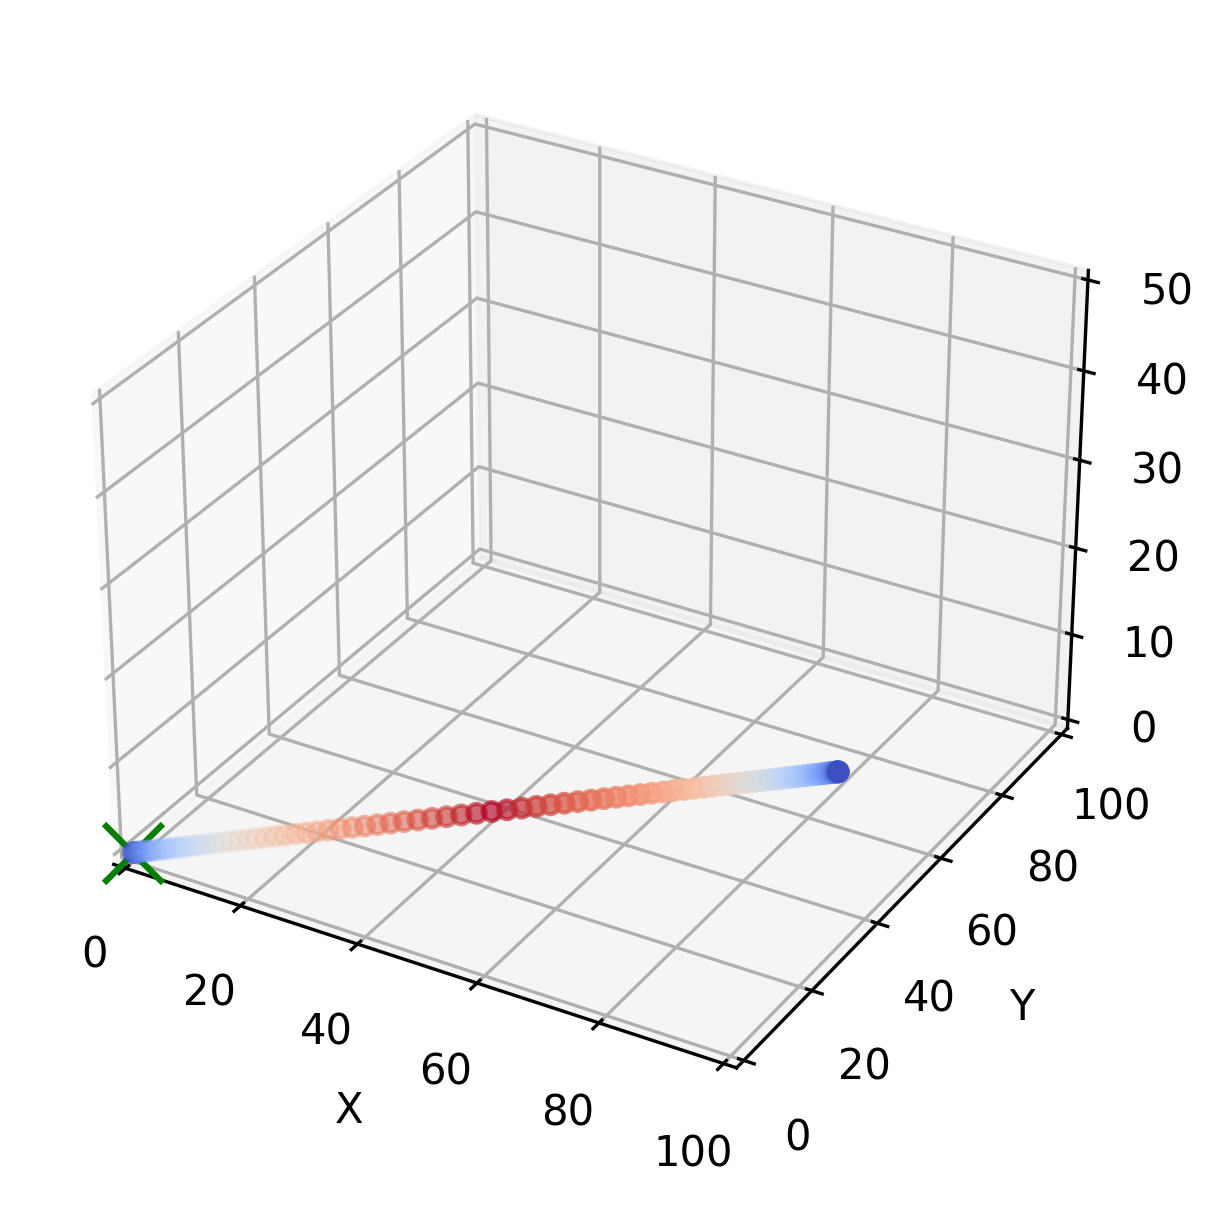
\includegraphics[width=\textwidth]{../python/output/test_single_cam_pos.png}
        \caption{Lineare Bewegung der Spidercam}
        \label{fig:length_change}
    \end{subfigure}
    \hfill
    \begin{subfigure}[b]{0.45\textwidth}
        \centering
        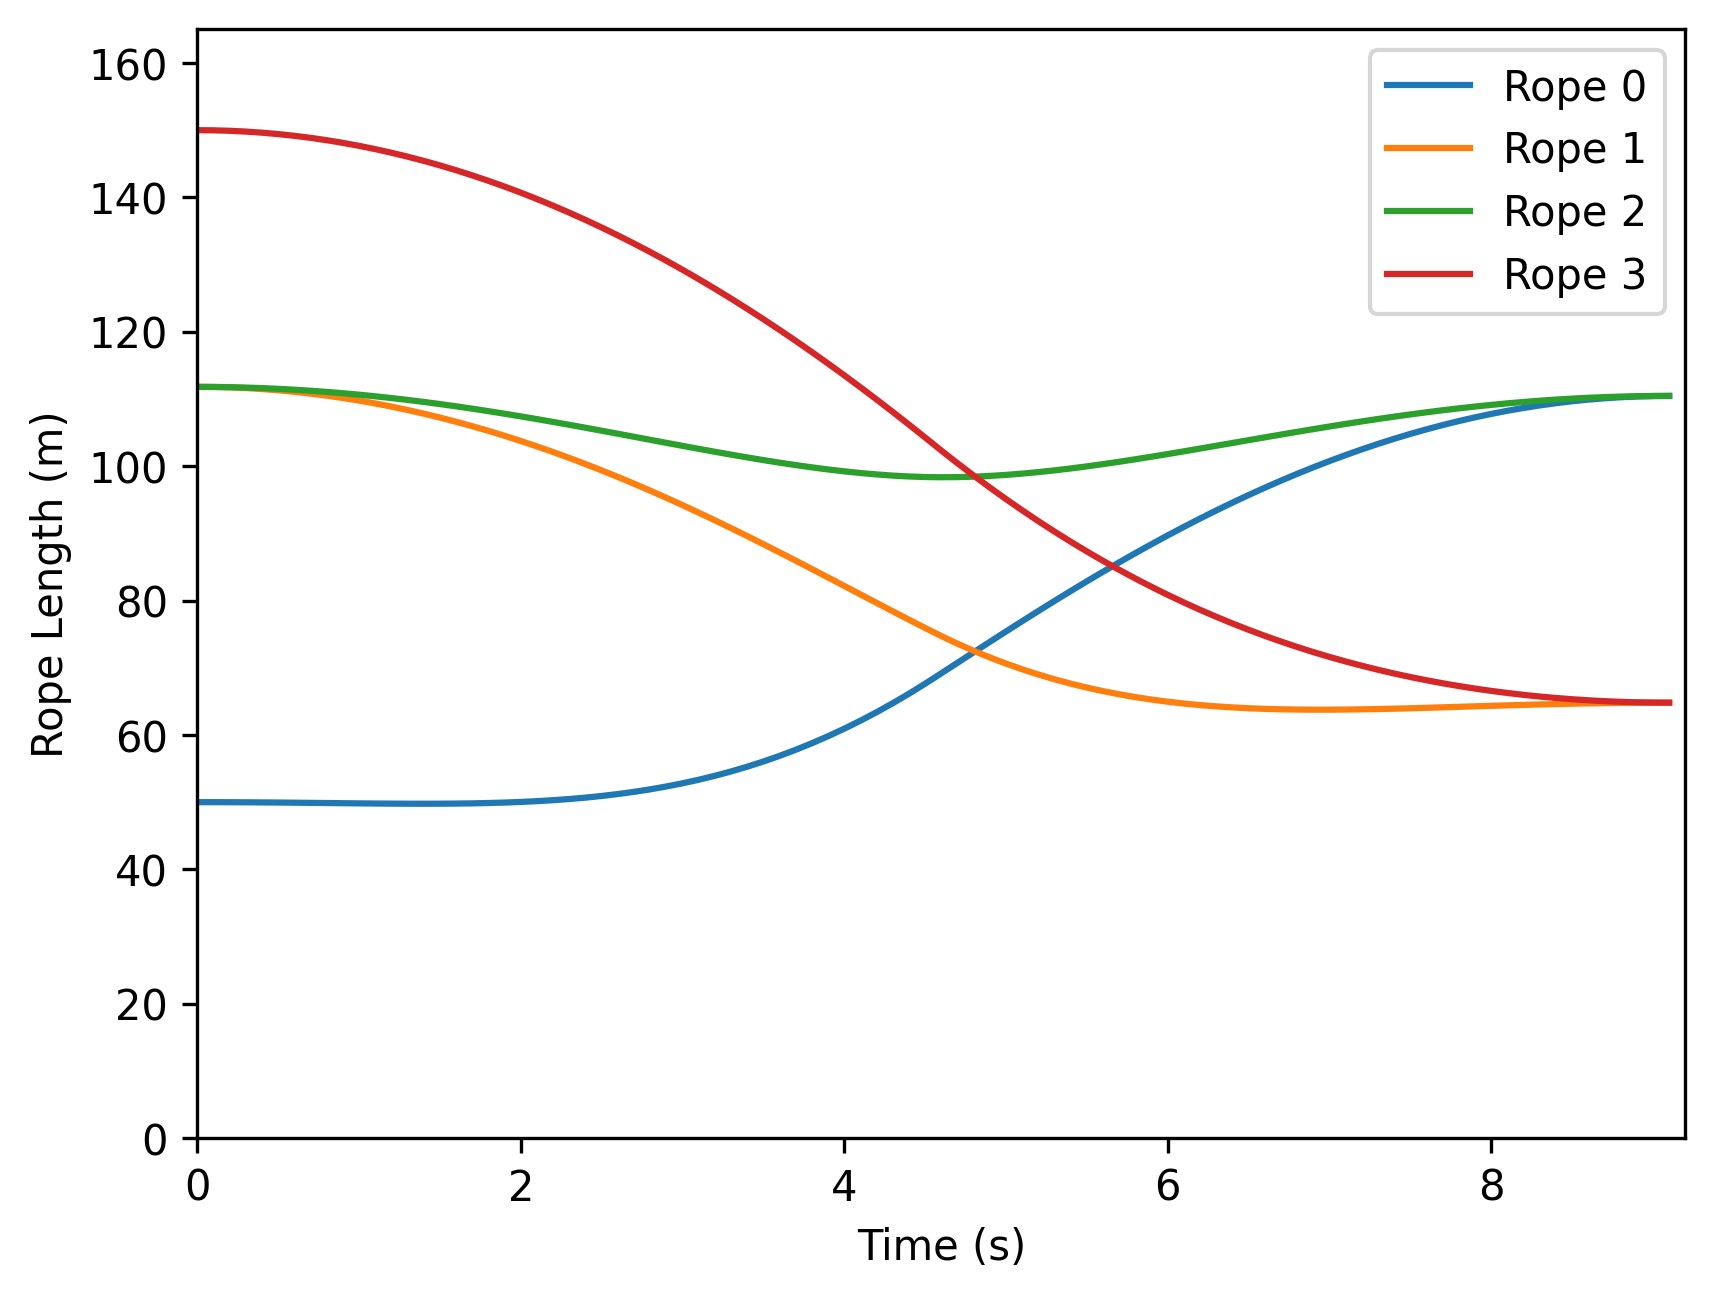
\includegraphics[width=\textwidth]{../python/output/test_single_rope_lengths.png}
        \caption{Veränderung der Seillängen}
        \label{fig:length_change_2}
    \end{subfigure}
    \caption{Beispiel für die Veränderung der Seillängen bei einer einfachen linearen Bewegung der Spidercam.
        Es ist zu erkennen, dass sich die Seillängen nicht linear verändern.
        Die Farbe der Bewegungspunkte gibt dabei an, wie schnell sich die Spidercam in diesem Moment bewegt.}
    \label{fig:length_change}
\end{figure}

Die einzelnen Punkte werden in den folgenden Abschnitten genauer erläutert.


\subsection{Eingabe}
\label{ssec:eingabe}

% Beschreibung der Eingabe

\subsubsection{Format}
\label{sssec:format}

% Beschreibung des Formats der Eingabe
Die Parameter für die Simulation einer Spidercam werden in Form einer Textdatei eingelesen.
Ein Beispiel für eine Eingabedatei ist in Abbildung \ref{fig:example_input} zu sehen.

% Path: figures/example_input.txt
\begin{figure}[H]
    \centering
    \lstinputlisting{figures/example_input.txt}
    \caption{Beispiel für eine Eingabedatei}
    \label{fig:example_input}
\end{figure}

% Beschreibung der Bedeutung der einzelnen Zeilen
Kommentare werden mit einem \# eingeleitet und dauern bis zum Ende der Zeile an.
Die Parameter werden in der Reihenfolge der folgenden Liste eingelesen\footnote{Von einer \emph{syntaktisch} korrekten Eingabedatei kann ausgegangen werden.}:
\begin{itemize}
    \item Dimension des Spielfelds (\texttt{dim x y z}),
    \item Startkoordinaten der Spidercam (\texttt{start x y z}),
    \item Maximalgeschwindigkeit der Spidercam (\texttt{vmax v}),
    \item (Maximal-)Beschleunigung der Spidercam (\texttt{amax a}),
    \item Diskretisierung der Bewegung (\texttt{freq f}),
    \item Beliebige Anzahl an Instruktionen mit Zeitpunkt und Zielkoodinaten (\texttt{t x y z}).
\end{itemize}

\subsubsection{Fehlerquellen und -behebung}
\label{sssec:fehlerquellen_und_-behebung}

% Beschreibung der Fehlerquellen
Die offensichtlichste Fehlerquellen sind:

\begin{itemize}
    \item Dimension besitzt nicht positive Werte
    \item Startposition außerhalb des Spielfelds
    \item Maximalgeschwindigkeit oder -beschleunigung sind nicht positiv
    \item Diskretisierung ist nicht positiv
    \item Instruktionen außerhalb des Spielfelds\footnote{Von chronologisch korrekt sortierten Instruktionen kann ausgegangen werden.}
\end{itemize}

% Beschreibung der Fehlerbehebung
Fehlerhafte Eingaben werden vor Initialisierung der Simulation abgefangen und mit einer Fehlermeldung beendet.


\subsection{Ausgabe}
\label{ssec:ausgabe}

% Beschreibung der Ausgabe

\subsubsection{Format}
\label{sssec:format}

% Beschreibung des Formats der Ausgabe
Für die Simulation sollen zwei CSV-Ausgabedateien erzeugt werden, die zu diskreten Zeitpunkten von $t = 0$ bis zum Zeitpunkt der Beendigung der letzten Instruktion $t_c$ die Längen der Drahtseile und die Positionen der Spidercam in der in der Eingabedatei angegebenen Frequenz $f \ [\si{\hertz} = \si{\per\second}]$ speichern.

Ausgabedatei 1 (siehe Abbildung \ref{fig:example_output_1}) enthält pro Zeile die Längen eines Seils zu jedem diskreten Zeitpunkt $t_i = i \cdot f^{-1}$, wobei $i \in [0, t_c \cdot f]$.
Für jeden Verankerungspunkt wird also eine Zeile angelegt.

Ausgabedatei 2 (siehe Abbildung \ref{fig:example_output_2}) enthält zeilenweise:
\begin{itemize}
    \item Dimension des Spielfelds,
    \item diskrete Zeitpunkte,
    \item $x$-Koordinate der Spidercam zu jedem Zeitpunkt $t_i$,
    \item $y$-Koordinate der Spidercam zu jedem Zeitpunkt $t_i$,
    \item $z$-Koordinate der Spidercam zu jedem Zeitpunkt $t_i$.
\end{itemize}

% Path: figures/example_output_1.txt
\begin{figure}[H]
    \centering
    \lstinputlisting{figures/example_output_1.txt}
    \caption{Beispiel für eine Ausgabedatei 1}
    \label{fig:example_output_1}
\end{figure}

% Path: figures/example_output_2.txt
\begin{figure}[H]
    \centering
    \lstinputlisting{figures/example_output_2.txt}
    \caption{Beispiel für eine Ausgabedatei 2}
    \label{fig:example_output_2}
\end{figure}

% % Beschreibung der Bedeutung der einzelnen Zeilen
% In der Ausgabedatei sollen also $\ldots$.

% \subsubsection{Fehlerquellen und -behebung}
% \label{sssec:fehlerquellen_und_behebung}

% % Beschreibung der Fehlerquellen
% Die offensichtlichste Fehlerquellen sind:

% \begin{itemize}
%     \item $\ldots$
%     \item $\ldots$
%     \item $\ldots$
% \end{itemize}

% % Beschreibung der Fehlerbehebung
% Um diese Fehlerquellen zu vermeiden, kann $\ldots$.

\subsection{Mathematische Modellierung}
\label{ssec:mathematische_modellierung}

\subsubsection{Berechnung der Seillängen}
\label{sssec:berechnung_der_seillaengen}

% Beschreibung der Berechnung der Seillängen
Die Verankerungspunkte der Drahtseile sind eindeutig durch die Dimension des Spielfeldes gegeben.
Es gilt:
\[
    R_1 = \begin{pmatrix}
        0 \\ 0 \\ d_z
    \end{pmatrix},
    \quad
    R_2 = \begin{pmatrix}
        d_x \\ 0 \\ d_z
    \end{pmatrix},
    \quad
    R_3 = \begin{pmatrix}
        0 \\ d_y \\ d_z
    \end{pmatrix},
    \quad
    R_4 = \begin{pmatrix}
        d_x \\ d_y \\ d_z
    \end{pmatrix}
\]

Die Längen der Drahtseile $l_i$ zu einem beliebigen Punkt im Raum $A = (x, y, z)$ sind dann trivialerweise gegeben durch:
\[
    l_i = d(R_i, A) = \| (R_i - A) \|_2 =
    \sqrt{
        (x - R_{i, x})^2 + (y - R_{i, y})^2 + (z - R_{i, z})^2
    }
\]

% Beschreibung der mathematischen Modellierung
\subsubsection{Bewegung der Spidercam}
\label{sssec:bewegung_der_spidercam}

% Beschreibung der Bewegung der Spidercam
Die Konstanten der Eingabedatei $a_{\max}$ und $v_{\max}$ werden hier als gegeben betrachtet.
Mithilfe dieser Konstanten können dann der Zeitraum $t_{\max}$ und die Distanz $d_{\max}$ berechnet werden, die die Spidercam in der Simulation benötigt, um die maximale Geschwindigkeit $v_{\max}$ zu erreichen.
Es gilt:
\[
    t_{\max} = \frac{v_{\max}}{a_{\max}} \quad \text{und} \quad d_{\max} = \frac{v_{\max}^2}{2 \cdot a_{\max}}
\]

Die maximale Geschwindigkeit $v_{\max}$ wird also nach $t_{\max}$ bzw. $d_{\max}$ erreicht.

Eine Bewegung der Spidercam ist dann eindeutig durch den Startpunkt $A$ und den Zielort $B$ gegeben.
Es können zwei Fälle unterschieden werden.

% Dreiphasige Bewegung
Eine \emph{dreiphasige Bewegung} tritt auf, wenn die Spidercam die maximale Geschwindigkeit $v_{\max}$ auf dem Weg von $A$ nach $B$ erreichen kann.

Es gilt($d(A, B) > 2 \cdot d_{\max}$)
\[
    \underbrace{(A)}_{\text{Start}} \rightarrow \underbrace{\left(A + \frac{d_{\max}}{d(A, B)} \cdot (B - A)\right)}_{\text{Zwischenpunkt}} \rightarrow \underbrace{\left(B - \frac{d_{\max}}{d(A, B)} \cdot (B - A)\right)}_{\text{Zwischenpunkt}} \rightarrow \underbrace{(B)}_{\text{Ziel}}
\]

\begin{figure}[H]
    \centering
    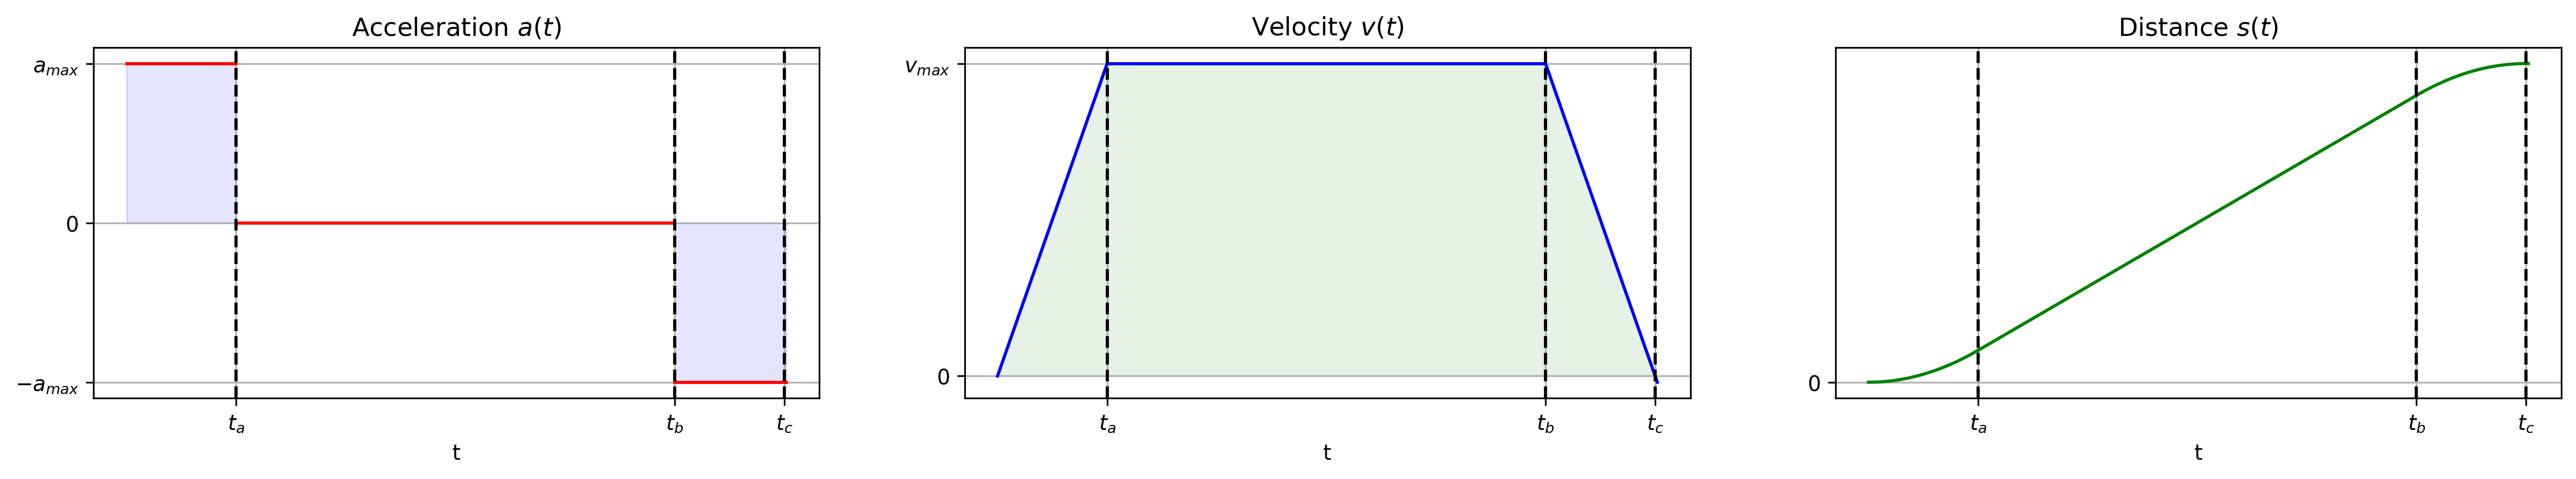
\includegraphics[width=\textwidth]{figures/three_phases.png}
    \caption{Bewegung der Spidercam in drei Phasen. $t_a$ entspricht dem Zeitraum, in dem die Spidercam maximal beschleunigt wird. $t_b$ ist der Zeitpunkt, an dem abgebremst wird und $t_c$ ist der Zeitpunkt, an dem die Spidercam ihren Zielort erreicht hat.}
    \label{fig:three_phases}
\end{figure}

Es gilt also, dass nach $t_{max}$ bzw. $d_{\max}$ der Zwischenpunkt $t_a$ erreicht wird, an dem die maximale Geschwindigkeit $v_{\max}$ erreicht ist.
Danach bewegt sich die Spidercam mit konstanter Geschwindigkeit $v_{\max}$ bis zum Zeitpunkt $t_b$, ab dem abgebremst werden muss, um am Zielort die Geschwindigkeit 0 zu erreichen.
Analog zum Beschleunigen benötigt die Spidercam zum Abbremsen auf 0 die Zeit $t_{\max}$ bzw. die Distanz $d_{\max}$.
Für die Phase der konstanten Geschwindigkeit gilt also:
\[
    d_{\CON} = d(A, B) - 2 \cdot d_{\max}
\]

Da die Geschwindigkeit konstant ist, gilt für die Zeit $t_{\CON}$ und damit $t_b$:
\[
    t_{\CON} = \frac{d_{\CON}}{v_{\max}} = \frac{d(A, B) - 2 \cdot d_{\max}}{v_{\max}} \implies t_b = t_{\max} + t_{\CON}
\]

Für diese Phase gilt damit (siehe auch Abbildung \ref{fig:three_phases}):
\[
    a(t) =
    \begin{cases}
        a_{\max}  & \text{für } 0 \leq t \leq t_a \\
        0         & \text{für } t_a < t \leq t_b  \\
        -a_{\max} & \text{für } t_b < t \leq t_c
    \end{cases}
\]

\[
    v(t) = \int_0^t a(u) \, \mathrm{d}u =
    \begin{cases}
        a_{\max} \cdot t                    & \text{für } 0 \leq t \leq t_a \\
        v_{\max}                            & \text{für } t_a < t \leq t_b  \\
        v_{\max} - a_{\max} \cdot (t - t_b) & \text{für } t_b < t \leq t_c
    \end{cases}
\]

\[
    s(t) = \int_0^t v(u) \, \mathrm{d}u =
    \begin{cases}
        \frac{a_{\max}}{2} \cdot t^2                                                      & \text{für } 0 \leq t \leq t_a \\
        s(t_a) + v_{\max} \cdot (t - t_a)                                                 & \text{für } t_a < t \leq t_b  \\
        s(t_a) + s(t_b) + v_{\max} \cdot (t - t_b) - \frac{a_{\max}}{2} \cdot (t - t_b)^2 & \text{für } t_b < t \leq t_c
    \end{cases}
\]

% Zweiphasige Bewegung
Eine \emph{zweiphasige Bewegung} (siehe Abbildung \ref{fig:two_phases}) tritt auf, wenn die Spidercam die maximale Geschwindigkeit $v_{\max}$ \emph{nicht} auf dem Weg von $A$ nach $B$ erreichen kann.

Es gilt ($d(A, B) \leq 2 \cdot d_{\max} $):
\[
    \underbrace{(A)}_{\text{Start}} \rightarrow \underbrace{\left(A + \frac{d(A, B)}{2} \cdot (B - A)\right)}_{\text{Zwischenpunkt}} \rightarrow \underbrace{(B)}_{\text{Ziel}}
\]

Es ist also direkt ersichtlich, dass eine Phase konstanter Geschwindigkeit entfällt.
Die höchste Geschwindigkeit in dieser Bewegung $v_x$ wird also aufgrund der gleich langen Beschleunigungs- und Abbremsphases genau zwischen $A$ und $B$ erreicht.
Die Zeit $t_x$ ist der Zeitpunkt, an dem die maximale Geschwindigkeit $v_{x}$ erreicht wird.

Es gilt also:
\[
    d_x = \frac{d(A, B)}{2} \implies t_x = \frac{d(A, B)}{2 \cdot v_{\max}} \implies v_x = a_{\max} \cdot t_x \left( = \frac{d_x}{t_x}\right)
\]


Die Berechnungen in dieser Form werden später auch in der Implementierung verwendet.

\begin{figure}[H]
    \centering
    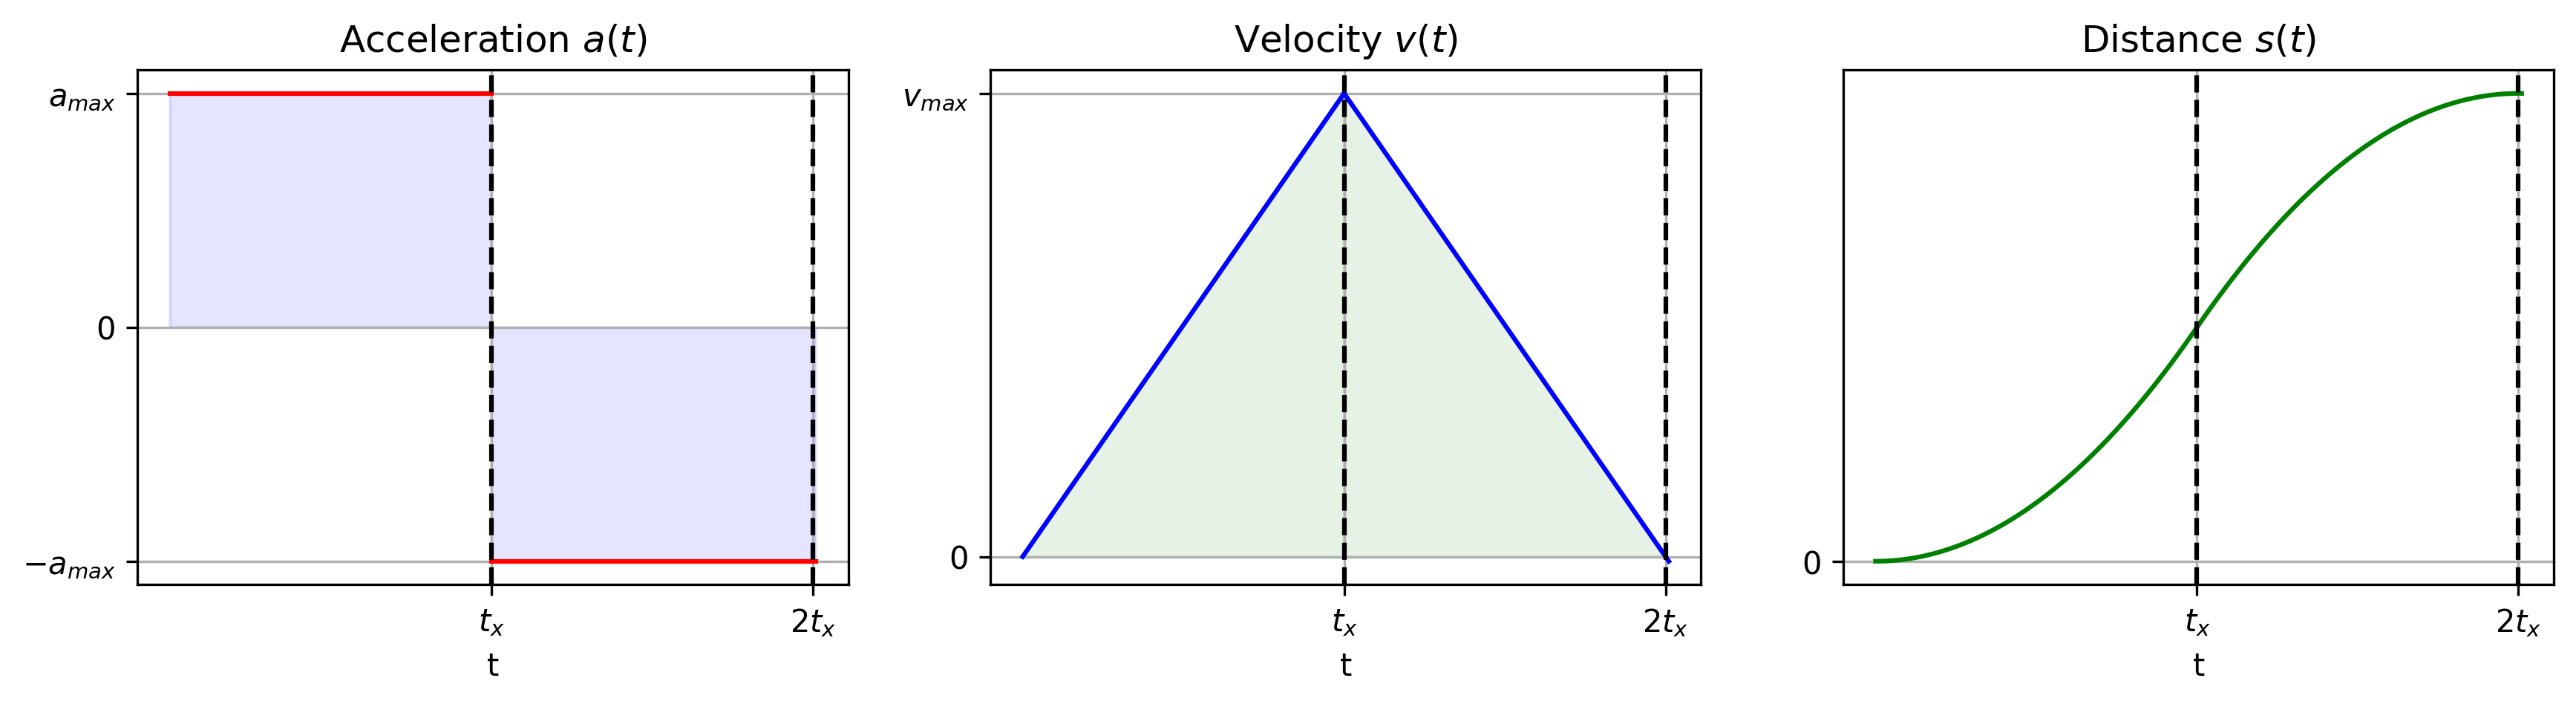
\includegraphics[width=\textwidth]{figures/two_phases.png}
    \caption{Bewegung der Spidercam in zwei Phasen. $t_x$ ist der Zeitpunkt, an dem abgebremst wird und $2t_x$ ist der Zeitpunkt, an dem die Spidercam ihren Zielort erreicht hat.}
    \label{fig:two_phases}
\end{figure}

\subsubsection{Abbrechen der Bewegung}
Instruktionen zur Bewegung der Spidercam können zu jedem Zeitpunkt stattfinden.
Befindet sich die Spidercam jedoch bereits in Bewegung während eine neue Instruktion ankommt, so wird die aktuelle Bewegung abgebrochen, indem die Spidercam sofort anfängt zu bremsen\footnote{Wenn bereits gebremst wird, muss nicht neu abgebremst werden.}.
Die neue Bewegung beginnt dann erst, wenn die Spidercam ihre Geschwindigkeit auf 0 gebracht hat.
Kommt eine neue Instruktion an, obwohl bereits eine Instruktion auf Ausführung wartet, so wird die alte Instruktion überschrieben, da diese als veraltet angenommen wird.



Für die weitere Implementierung ist es hier wichtig zu klären, wie sich die Bremsdistanz $d_{\DEC}$, die Bremszeit $t_{\DEC}$ und das neue Ziel $B'$ bestimmen lassen.

Die Bremsdistanz $d_{\DEC}$ ist die Distanz, die die Spidercam zurücklegt, wenn sie von ihrer aktuellen Geschwindigkeit $v$ auf 0 abgebremst wird.
Die Bremsdistanz ist also gleich der Fläche unter der Geschwindigkeitskurve $v(t)$.
Die Fläche unter der Kurve $v(t)$ ist die Distanz, die die Spidercam zurücklegt (siehe Abbildung \ref{fig:forced_deceleration}).

\begin{figure}[H]
    \centering
    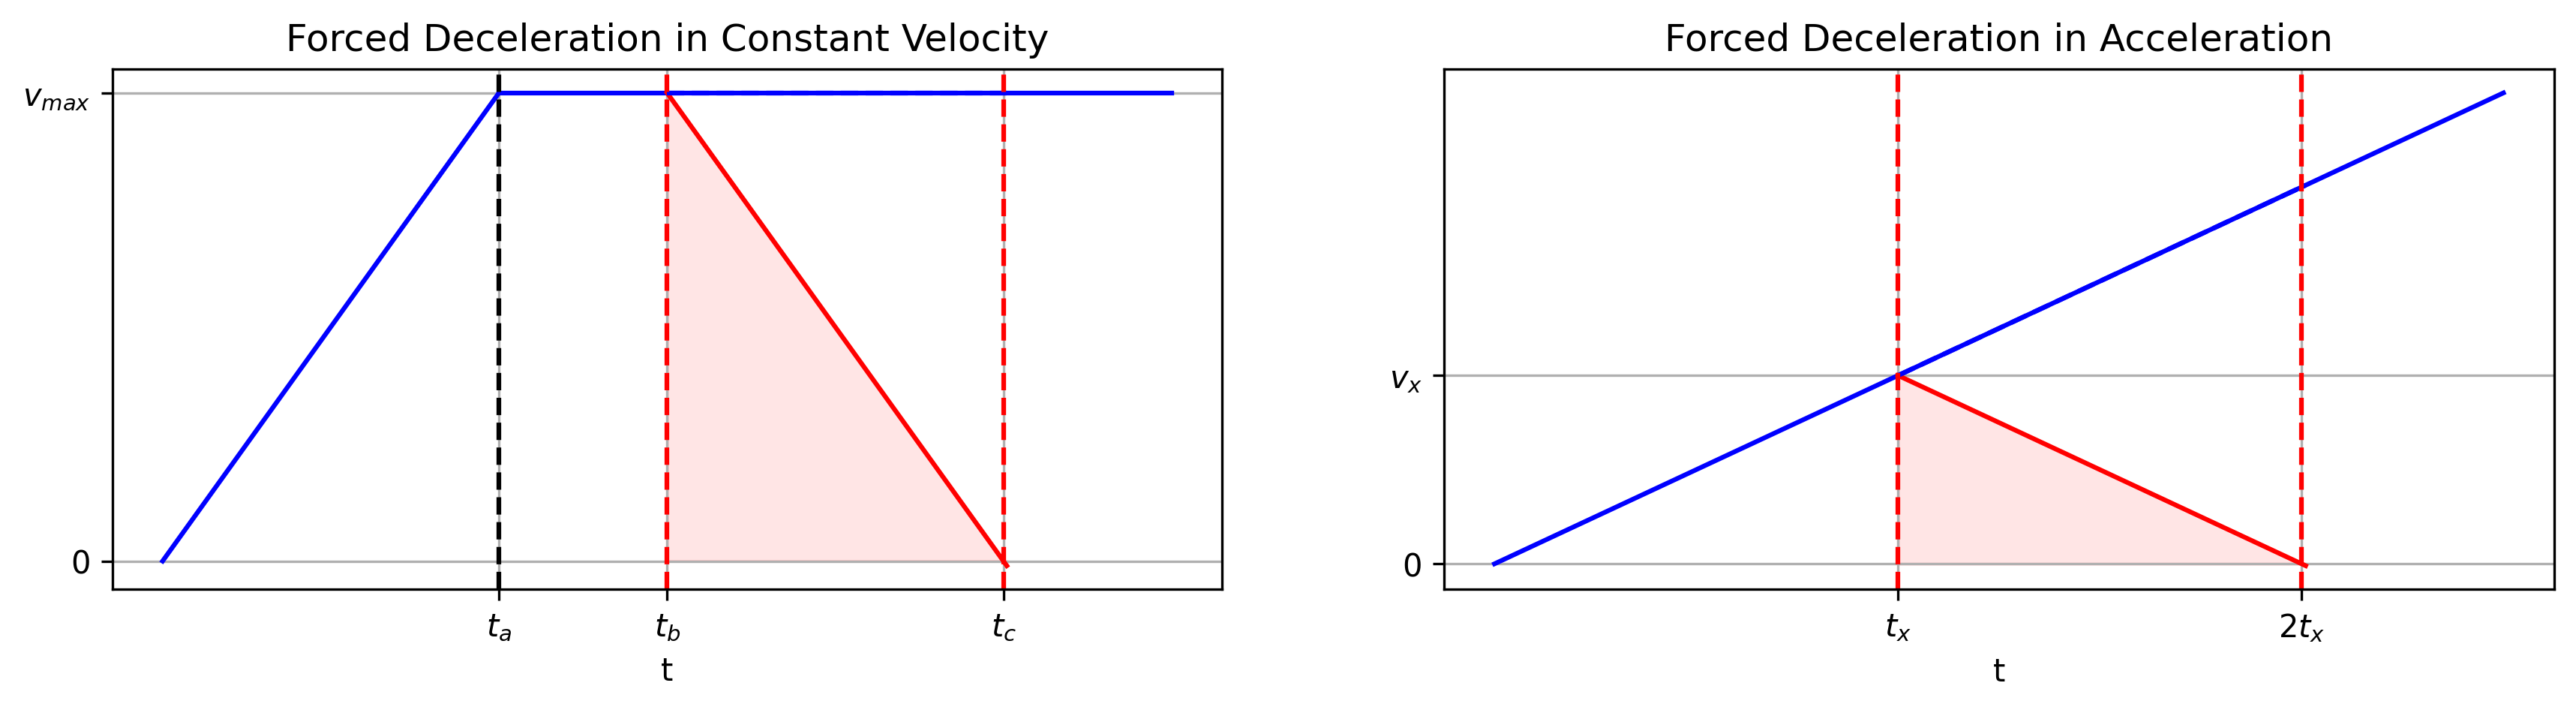
\includegraphics[width=\textwidth]{figures/forced_deceleration.png}
    \caption{Berechnung der Bremsdistanz $d_{\DEC}$}
    \label{fig:forced_deceleration}
\end{figure}

Da die Beschleunigung konstant ist, gilt:
\[
    v(t) = \begin{cases}
        v_{\max}         & \text{für Abbruch in Phase konstanter Geschwindigkeit} \\
        a_{\max} \cdot t & \text{für Abbruch in Beschleunigungsphase}
    \end{cases}
\]

Damit lassen sich dann die Bremszeit $t_{\DEC}$ und die Bremsdistanz $d_{\DEC}$ berechnen:

\[
    t_{\DEC} = \frac{v(t)}{a_{\max}} \implies d_{\DEC} = \frac{v(t)^2}{2 \cdot a_{\max}}
\]

Die neue Position $B'$ ist der Punkt, an dem die Spidercam anhalten würde, wenn sie von ihrer aktuellen Position $A$ für die Bremsdistanz $d_{\DEC}$ in Richtung $B$ fahren würde.
Dazu wird der Vektor $(B - A)$ normiert und mit der Bremsdistanz $d_{\DEC}$ multipliziert:
\[
    B' = A + \frac{d_{\DEC}}{d(A, B)} \cdot (B - A)
\]